\cleardoublepage
\begin{minipage}{0.95\linewidth}
  \part{Introduction}
  \vspace{15mm} % l'espacement souhaité
  \parttoc 
\end{minipage}

\chapter{Ordonnancement, ressources cumulatives et énergie}

Dans ce chapitre, nous commençons par définir ce qu'est un problème
d'ordonnancement et quelles sont les principales caractéristiques de
ces problèmes. Ensuite, nous présenterons deux exemples de problèmes
d'ordonnancement cumulatifs que nous utiliserons tout au long de ce
manuscrit, le problème d'ordonnancement de projet à contraintes de
ressources (RCPSP) et le problème cumulatif (CuSP). Nous montrerons
ensuite les limites de ces problèmes en termes de modélisation des
modalités d'utilisation de certaines ressources et nous introduirons une nouvelle 
extension du CuSP, le problème d'ordonnancement continu à contraintes
énergétiques (CECSP), pour pallier ces limites. Cette nouvelle
extension sera ensuite comparée aux extensions existantes du \RCPSP~et
du \CUSP.  Enfin, plusieurs propriétés du \CECSP, qui seront utilisées
dans la suite de ce manuscrit, seront présentées.


\section{Ordonnancement et contraintes de ressources}
\label{sec:ordo}
\subsection{L'ordonnancement}
\label{sec:ordo_def}
La théorie de l'ordonnancement s'intéresse au calcul de dates
d'exécution d'un ensemble d'activités. Dans cette optique,
l'utilisation d'une ou plusieurs ressources peut être nécessaire et
l'exécution d'une activité implique souvent une telle consommation. Un
problème d'ordonnancement peut alors être vu comme l'organisation dans
le temps de la réalisation d'activités soumises à des contraintes de
temps et de ressource. Dans la plupart des cas, un ou plusieurs
objectifs sont définis et une solution au problème d'ordonnancement 
vise à optimiser ces objectifs.
 
\subsubsection{Les activités}

Une activité peut être définie par une date de début $st_i$ et une date
de fin $et_i$ et une durée $p_i$ vérifiant $et_i=st_i+p_i$. Si
l'activité utilise une ou plusieurs ressources durant son exécution, il
est nécessaire d'ajouter à cette définition une fonction d'allocation
de ressource propre à chaque activité $i$ et à chaque
ressource $k$. Si cette fonction est donnée dans les paramètres du
problème, on la note $r_{ik}(t)$. Si, au contraire, elle fait partie
des variables de décision du problème, on la note $b_{ik}(t)$. Enfin,
si cette fonction ne dépend pas du temps, i.e. est constante, le
paramètre $t$ pourra être omis. 

Selon les problèmes, une activité peut être contrainte à s'exécuter en
un seul morceau. On parle alors d'activité non préemptive et dans le
cas contraire, i.e. les activités peuvent être exécutées en plusieurs
morceaux, on parle d'activité préemptive.

Une activité peut être utilisée pour représenter, par exemple, une
opération dans un processus de production, le décollage/atterrissage
d'un avion ou encore une étape d'un projet de construction.

\subsubsection{Les ressources}

Une ressource $k$ est un moyen technique ou humain requis pour la
réalisation d'une activité et est disponible en quantité
limitée. Cette quantité, appelée {\it disponibilité de la ressource ou
  capacité}, peut être soit constante ou varier au cours du
temps. Dans ce manuscrit, nous considérons des ressources à capacité
constante et cette capacité est notée $R_k$. Les ressources utilisées
par les activités peuvent être de nature diverse. Parmi elles, on peut
distinguer:
\begin{itemize}
\item les ressources renouvelables: ces ressources peuvent être
réutilisées dès lors qu'elles sont libérées. Il s'agit, en fait, de
ressources qui, après avoir été utilisées par une ou plusieurs
activités, sont de nouveau disponible en même quantité. Ces ressources
peuvent, par exemple, représenter la main d'\oe uvre d'une entreprise,
des machines, de l'électricité ou des équipements.
\item à l'inverse, les ressources consommables sont des ressources
dont la consommation globale est limitée au cours du temps. Il peut
s'agir, par exemple, de matières premières ou d'un budget.
\end{itemize}

Parmi les ressources renouvelables, on distingue par ailleurs, les
ressources disjonctives qui ne peuvent exécuter qu'une activité à la
fois -- e.g. pistes de décollage, salles -- et les ressources cumulatives
qui peuvent, elles,  être utilisées par plusieurs activités en
parallèle mais sont disponibles en quantité limitée -- e.g. main d'\oe
uvre,
processeurs.


Du point de vue de leur divisibilité, les ressources peuvent aussi
être divisées selon deux catégories: 
\begin{itemize}
\item les ressources continues, i.e. divisibles en temps ou en
  quantité continu: dans le premier cas, il s'agit de ressources
  pouvant être ré-allouées à tout instant $t \in [0,T]$, où $T$ est une
  borne supérieure sur la date de fin de l'ordonnancement; dans le
  second cas, il s'agit de ressources pouvant être allouées en quantité
  continue, i.e. non discrète. Ce type de ressource permet, par
  exemple, de modéliser l'électricité, l'essence, l'énergie hydraulique...
\item les ressources discrètes, i.e. divisibles en temps ou en quantité
  discret: à l'inverse, le premier cas décrit une ressource où la
  ré-allocation de cette dernière ne peut être 
  exécutée qu'à des temps discrets $t \in \{0,\dots,T\}$; le second
  cas correspond aux ressources ne pouvant être attribuées aux
  activités qu'en quantité discrète,  e.g. employés, machines...
\end{itemize}

\subsubsection{Les contraintes}

Une contrainte permet d'exprimer des restrictions sur les valeurs que
peuvent prendre une ou plusieurs variables du problème. Parmi les
principales, on distingue:
\begin{itemize}
\item les contraintes de temps: elles intègrent les contraintes de
  temps alloué, issues généralement d'impératifs de gestion et
  relatives aux dates limites des activités (e.g. dates
    de livraison) ou à la durée totale d'un projet mais aussi les
    contraintes d'enchaînement qui décrivent des
    positionnements relatifs devant être respectés entre les
    activités. Ces contraintes peuvent, par exemple, modéliser des
    contraintes de précédence entre les activités, i.e. une activité
    ne peut commencer avant qu'une autre n'ait été achevée, ou des temps
    de transition à respecter entre les activités.

    {\'E}tant donné une activité $i$, la date à partir de laquelle
    l'activité $i$ peut être exécutée est appelée {\it date de début au
      plus tôt} et est notée $\ES$ (earliest start time en anglais). De
    même, la date avant laquelle l'activité $i$ doit avoir été
    complètement exécutée sera appelée {\it date de fin au plus tard} et
    notée $\LE$ (latest end time en anglais).

\item les contraintes de ressources:  ce sont des contraintes d'utilisation
  des ressources qui expriment la nature et la quantité de moyens
  utilisés par les activités, ainsi que les caractéristiques
  d'utilisation de ces moyens. Ces contraintes peuvent aussi représenter
  des contraintes de disponibilité des ressources qui précisent la
  nature et la quantité de moyens disponibles au cours du temps.
\end{itemize}

\subsubsection{Les objectifs}

Lors de la résolution d'un problème d'ordonnancement, deux buts
différents peuvent être poursuivis. Le premier vise à trouver une solution
réalisable pour le problème tandis que le second cherche à trouver une
solution optimisant un ou plusieurs critères ou objectifs.

Ces objectifs peuvent être liés à différents aspect de la solution. On
distingue par exemple:
\begin{itemize}
\item les objectifs liés au temps: le temps total d'exécution ou le temps moyen
  d'achèvement d'un ensemble d'activités peuvent être minimisés, mais
  aussi  les retards (maximum, moyen, somme...) par rapport
  aux dates de fin au plus tard fixées par le problème.
\item les objectifs liés aux ressources: la quantité (maximale,
  moyenne, pondérée...) de ressources nécessaires pour réaliser un
  ensemble d'activités peut, par exemple, être minimisée.
\item les objectifs liés aux coûts de lancement, de production, de
  transport, de stockage ou liés aux revenus, aux retours
  d'investissements... 
\item les objectifs liés à une énergie, un débit...
\end{itemize}

Deux exemples de problèmes d'ordonnancement sont présentés dans le
paragraphe suivant: le \RCPSP~et le \CUSP.

\section{Contraintes de ressource et contraintes }

Dans ce manuscrit, nous sommes principalement intéressé aux problèmes
d'ordonnancement cumulatifs. Parmi ces derni

\subsection{Problèmes cumulatifs}
\subsubsection{Le problème d'ordonnancement  de projet à contraintes de
  ressources}
\index{\RCPSPidx}
Le problème d'ordonnancement de projet à contraintes de ressources
(\RCPSP) est un problème d'ordonnancement très général, utilisé pour
modéliser de nombreux problèmes pratiques. L'objectif est
d'ordonnancer un ensemble d'activités de telle sorte que la capacité
de la ressource ne soit pas excédée et qu'une certaine fonction
objectif soit minimisée. Parmi les ressources modélisées, on trouve
des ressources telles que des machines, des personnes, des salles, de
l'argent ou encore de l'énergie. Pour les fonctions objectifs, des
quantités telles que la durée totale du projet, le retard ou les coûts
peuvent être minimiser.

Formellement, le \RCPSP~est défini de la manière suivante: nous
considérons un ensemble d'activités non-préemptives
$\A=\{1,\dots,n\}$ à ordonnancer et un ensemble $\R$ de ressources
renouvelables. Chacune de ces ressources $k \in \R$ est disponible
tout au long du projet en quantité $R_k$ et, durant son exécution, une
activité consomme une quantité $r_{ik}$ (pouvant être nulle) de cette
ressource. Dans ce problème, une activité $i \in \A$ a une durée fixe
$p_i$ et des relations de précédence lient les activités entre
elles. Ces relations sont souvent modélisées à l'aide d'un graphe
$G=(V,E)$, appelé graphe de précédence, dans lequel l'ensemble des
arcs $(i,j) \in E$ représente les relations de précédence, i.e. $(i,j)
\in E \Leftrightarrow i $ doit être ordonnancer avant $j$ dans toute
solution. Dans ce graphe, l'ensemble des sommets, dénoté par
$V=\{0,\dots,n+1\}$, correspond aux $n$ activités auxquelles on ajoute
deux activités fictives $0$ et $n+1$ qui représentent respectivement
le début et la fin du projet. Ces activités fictives ne consomment pas
de ressource et ont une durée d'exécution nulle. De plus, $E$ contient
les arcs suivants: 
\begin{itemize}
\item $(0,i),\ \forall i \in \A$,
\item $(i,n+1),\ \forall i \in \A$.
\end{itemize}

Pour ce problème, la fonction objective la
plus rencontrée dans la littérature étant la minimisation de la date
de fin du projet, i.e. $C_{max}$, nous considérons principalement cet
objectif dans la suite de ce manuscrit. Si un objectif différent est
considéré, nous le précisons. 

L'objectif du problème est donc de déterminer la date de début $st_i$
de chaque activité $i\in \A$ de telle sorte que:
\begin{itemize}
\item à chaque instant $t$, la somme, pour chaque activité, des
  consommations d'une même ressource $k \in \R$ ne doit pas dépasser la
  capacité $R_{k}$ de cette dernière, i.e.
  \begin{equation}\forall t \in \H, \forall k \in \R,\sum_{\substack{i\in \A\\ t \in
        [st_i,st_i+p_i]}} r_{ik} \le R_k\end{equation} 
  avec $\H=\{0,\dots,T\}$ défini l'horizon de temps du projet, où $T$
  est une borne supérieure sur la date de fin du projet.
\item les contraintes de précédences sont satisfaites, i.e. 
  \begin{equation} \forall (i,j) \in E,\ s_i+p_i \le p_j \end{equation}
\item la date de fin du projet $C_{max}= \max_{i \in \A} s_i+p_i$
  soit minimale. 
\end{itemize}

\begin{ex}
  \label{ex_RCPSP}
  Considérons l'instance à quatre activités et deux ressources suivante:
  \begin{itemize}
  \item $R_1=5$ et $R_2=7$
  \item cf. figure~\ref{instance_ex_RCPSP}
  \end{itemize}
  \begin{figure}[!htb]
    \centering
    \subcaptionbox{Données de l'instance de l'exemple du \RCPSP.}{
      \begin{tabular}{|P{1cm}|P{1cm}P{1cm}P{1cm}|}
        \hline
        i & p_i & r_{i1} & r_{i2}\\
        \hline
        1 & 4 & 2 & 3 \\
        2 & 3 & 1 & 5 \\
        3 & 5 & 2 & 2 \\
        4 & 8 & 2 & 4 \\
        \hline
      \end{tabular}}
    \hfill
    \subcaptionbox{Graphe de précédence de l'instance de
      l'exemple du \RCPSP.}{
      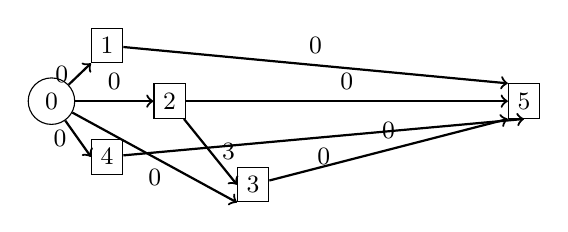
\begin{tikzpicture}
        [xscale=1.3]
        \node[draw,circle] (O) at (0,0) {\small $0$};
        \node[right of=O,draw,node distance=1.5cm] (D) {\small $2$}; 
        \node[above right of=O,draw] (U) {\small $1$}; 
        \node[below right of=D,draw,node distance =1.5cm] (T) {\small $3$}; 
        \node[below right of=O,draw] (Q) {\small $4$};
        \node[right of=D,draw,node distance=4.5cm] (C) {\small $5$};  

        \draw[->,thick] (O) -- (U.south west) node[midway, left=0.5pt] {\small $0$};
        \draw[->,thick] (O) -- (D.west) node[midway, above=0.5pt] {\small $0$};
        \draw[->,thick] (O) -- (T.south west) node[midway, below=0.5pt] {\small $0$};
        \draw[->,thick] (O) -- (Q.west) node[midway, left=0.5pt] {\small $0$};
        \draw[->,thick] (U) -- (C.north west) node[midway, above=0.5pt] {\small $0$};
        \draw[->,thick] (D) -- (C.west) node[midway, above=0.5pt] {\small $0$};
        \draw[->,thick] (D) -- (T.west) node[midway, right=0.5pt] {\small $3$};
        \draw[->,thick] (T) -- (C.south west) node[midway, above=0.5pt] {\small $0$};
        \draw[->,thick] (Q) -- (C.south) node[midway, below=0.5pt] {\small $0$};
      \end{tikzpicture}}
    \caption{Instance de l'exemple du \RCPSP.} 
    \label{instance_ex_RCPSP}
  \end{figure}

  La figure~\ref{solution_ex_RCPSP_feas} présente un ordonnancement
  réalisable avec $C_{max}=15$. Cet ordonnancement n'est pas optimal
  puisque si l'activité $1$ est décalée à droite de manière à commencer
  au temps $t=8$, on obtient un ordonnancement ayant une date de fin
  inférieure à celle de l'ordonnancement précédent, i.e. $C_{max}=12$
  (cf. figure~\ref{solution_ex_RCPSP_opt}).

  \begin{figure}[!htb]
    \centering
    \subcaptionbox{Une solution réalisable\label{solution_ex_RCPSP_feas}}[0.4\linewidth]{
      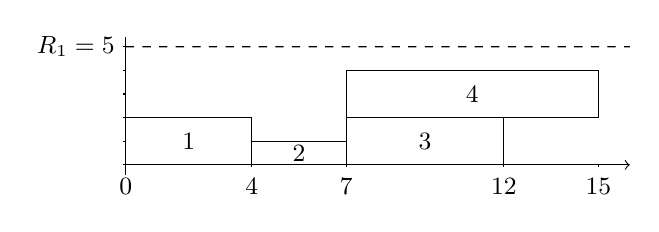
\begin{tikzpicture}
        [xscale=0.4,yscale=0.3]
        \node (O) at (0,0) {};
        \node (bmax) at (0,5) {};

        \draw[->] (O.center) -- (16,0);
        \draw (O.south) -- (bmax.north);

        \draw[dashed] (bmax.center) node[left=0.5pt] {\small $R_1=5$} -- (16,5);
        \draw[fill=white] (0,0) rectangle (4,2) node[midway] {\small $1$};
        \draw[fill=white] (4,0) rectangle (7,1) node[midway] {\small $2$};
        \draw[fill=white] (7,0) rectangle (12,2) node[midway] {\small $3$};
        \draw[fill=white] (7,2) rectangle (15,4) node[midway] {\small $4$};

        \draw (0,0) -- (0,-0.1) node[below=0.5pt] {\small $0$};
        \draw (4,0) -- (4,-0.1) node[below=0.5pt] {\small $4$};
        \draw (7,0) -- (7,-0.1) node[below=0.5pt] {\small $7$};
        \draw (12,0) -- (12,-0.1) node[below=0.5pt] {\small $12$};
        \draw (15,0) -- (15,-0.1) node[below=0.5pt] {\small $15$};

        \foreach \i in {0,...,5}
        {\draw (0,\i) -- (-0.1,\i);}
      \end{tikzpicture}

      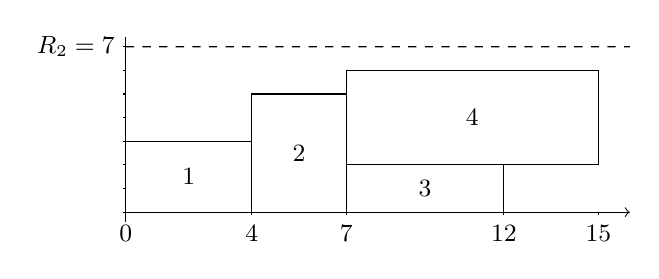
\begin{tikzpicture}
        [xscale=0.4,yscale=0.3]
        \node (O) at (0,0) {};
        \node (bmax) at (0,7) {};

        \draw[->] (O.center) -- (16,0);
        \draw (O.south) -- (bmax.north);

        \draw[dashed] (bmax.center) node[left=0.5pt] {\small $R_2=7$} -- (16,7);
        \draw[fill=white] (0,0) rectangle (4,3) node[midway] {\small $1$};
        \draw[fill=white] (4,0) rectangle (7,5) node[midway] {\small $2$};
        \draw[fill=white] (7,0) rectangle (12,2) node[midway] {\small $3$};
        \draw[fill=white] (7,2) rectangle (15,6) node[midway] {\small $4$};

        \draw (0,0) -- (0,-0.1) node[below=0.5pt] {\small $0$};
        \draw (4,0) -- (4,-0.1) node[below=0.5pt] {\small $4$};
        \draw (7,0) -- (7,-0.1) node[below=0.5pt] {\small $7$};
        \draw (12,0) -- (12,-0.1) node[below=0.5pt] {\small $12$};
        \draw (15,0) -- (15,-0.1) node[below=0.5pt] {\small $15$};

        \foreach \i in {0,...,7}
        {\draw (0,\i) -- (-0.1,\i);}
      \end{tikzpicture}}
    \hfill
    \subcaptionbox{La solution optimale\label{solution_ex_RCPSP_opt}}[0.4\linewidth]{
      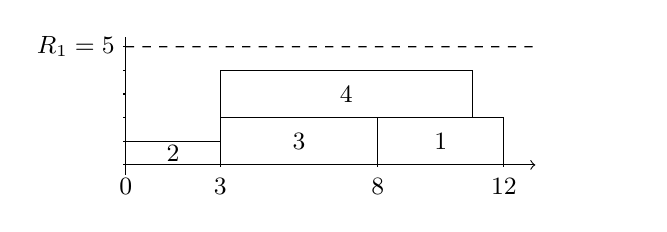
\begin{tikzpicture}
        [xscale=0.4,yscale=0.3]
        \node (O) at (0,0) {};
        \node (bmax) at (0,5) {};
        \node at (16,0) {};
        \draw[->] (O.center) -- (13,0);
        \draw (O.south) -- (bmax.north);

        \draw[dashed] (bmax.center) node[left=0.5pt] {\small $R_1=5$} -- (13,5);
        \draw[fill=white] (0,0) rectangle (3,1) node[midway] {\small $2$};
        \draw[fill=white] (3,0) rectangle (8,2) node[midway] {\small $3$};
        \draw[fill=white] (3,2) rectangle (11,4) node[midway] {\small $4$};
        \draw[fill=white] (8,0) rectangle (12,2) node[midway] {\small $1$};

        \draw (0,0) -- (0,-0.1) node[below=0.5pt] {\small $0$};
        \draw (3,0) -- (3,-0.1) node[below=0.5pt] {\small $3$};
        \draw (8,0) -- (8,-0.1) node[below=0.5pt] {\small $8$};
        \draw (12,0) -- (12,-0.1) node[below =0.5pt] {\small $12$};

        \foreach \i in {0,...,5}
        {\draw (0,\i) -- (-0.1,\i);}
      \end{tikzpicture}

      \begin{tikzpicture}
        [xscale=0.4,yscale=0.3]
        \node (O) at (0,0) {};
        \node (bmax) at (0,7) {};
        \node at (16,0) {};

        \draw[->] (O.center) -- (13,0);
        \draw (O.south) -- (bmax.north);

        \draw[dashed] (bmax.center) node[left=0.5pt] {\small $R_2=7$} -- (13,7);
        \draw[fill=white] (0,0) rectangle (3,5) node[midway] {\small $2$};
        \draw[fill=white] (3,3) rectangle (11,7) node[midway] {\small $4$};
        \draw[fill=white] (3,0) rectangle (8,2) node[midway] {\small $3$};
        \draw[fill=white] (8,0) rectangle (12,3) node[midway] {\small $1$};

        \draw (0,0) -- (0,-0.1) node[below=0.5pt] {\small $0$};
        \draw (3,0) -- (3,-0.1) node[below=0.5pt] {\small $3$};
        \draw (8,0) -- (8,-0.1) node[below=0.5pt] {\small $8$};    
        \draw (12,0) -- (12,-0.1) node[below=0.5pt] {\small $12$};

        \foreach \i in {0,...,7}
        {\draw (0,\i) -- (-0.1,\i);}
      \end{tikzpicture}}
    \caption{Deux solutions réalisables pour l'exemple du \RCPSP.} 
    \label{solution_ex_RCPSP}
  \end{figure}
\end{ex}

Le \RCPSP~est un problème qui a été prouvé NP-complet au sens
fort~\cite{NP_RCPSP}. Ce problème a donc été très étudié dans la
littérature, notamment pour trouver des méthodes efficaces pour sa
résolution. Dans la section~\ref{sec:PLNE_ordo_res}, nous présentons des
modèles de programmation linéaire permettant de trouver la solution
optimale à ce problème. 

\subsubsection{Le problème cumulatif}

En ordonnancement avec contraintes de ressources, on distingue deux
types de ressources:
\begin{itemize}
\item les ressources disjonctives qui ont la particularité que, à un
  instant $t$, une et une seule activité peut utiliser la ressource.
\item à l'inverse, les ressources cumulatives se distinguent par le
  fait que plusieurs activités peuvent utiliser la ressource
  simultanément à la condition que la consommation totale n'excède pas
  la capacité de la ressource.
\end{itemize}
Le problème d'ordonnancement cumulatif (CuSP)\index{\CuSPidx} permet
de caractériser le fait qu'une ressource (ou un sous-ensemble) soit de
type cumulative dans un projet. Il s'agit en fait d'un cas particulier
du \RCPSP.

Formellement, le \CUSP~prend en entrée un ensemble $
\A=\{1,\dots,n\}$ d'activités non-préemptives à ordonnancer. Pour s'exécuter, une
activité doit consommer une partie de la ressource $r_i$ et ce jusqu'à
l'arrêt de celle-ci, i.e. après un temps $p_i$ correspondant à la
durée de l'activité $i$. Cette ressource est de type cumulative et
renouvelable, disponible en quantité $R$. 

De plus, chaque activité dispose d'une fenêtre de temps $[\ES,\LE]$
dans laquelle l'activité doit obligatoirement s'exécuter. On appelle $\ES$ 
la date de début au plus tôt de $i$ et $\LE$ sa date de
fin au plus tard. 

L'objectif du \CUSP~est donc de déterminer la date de début $st_i$ de
chaque activité $i \in \A$ telle que:
\begin{itemize}
\item la capacité de la ressource n'est excédée à aucun moment du
  projet, i.e.
  \begin{equation} \forall t \in \H,\sum_{\substack{i\in \A\\ t \in
        [st_i,st_i+p_i]}} r_{i} \le  R\end{equation}
  où $\H=\{0,\dots,T\}$ est l'horizon de temps du projet et $T=\max_{i
    \in \A} \LE$.
\item la fenêtre de temps de chaque activité est respectée, i.e. 
  \begin{equation} \forall i \in \A,\ \ES \le st_i < st_i+p_i \le \LE \end{equation}
\end{itemize}

Trouver une solution réalisable pour ce problème - étant
une extension de la variante de décision du problème à une machine
($R=1$ et $r_i=1$) et du problème à $m$ machines ($R=m$ et $r_i=1$) - 
est NP-complet au sens fort~\cite{NP_bible}. De ce fait, dans la
littérature, ce problème est souvent étudié sans fonction
objectif. Sauf précision du contraire, nous ferons de même dans la
suite du manuscrit. 

\begin{ex}
  \label{CUSP_ex}
  Considérons l'instance à quatre activités suivante:
  \begin{itemize}
  \item $R=4$
  \item cf. table~\ref{instance_CUSP_ex}\begin{table}[!htb]
      \centering
      \begin{tabular}{|P{1cm}|P{1cm}P{1cm}P{1cm}P{1cm}|}
        \hline
        i & p_i & \ES & \LE & r_i\\
        \hline
        1 & 2 & 1 & 5 & 2 \\
        2 & 1 & 3 & 5 & 2\\
        3 & 1 & 3 & 5 & 3\\
        4 & 4 & 1 & 10 & 1 \\
        \hline
      \end{tabular}
      \caption{Données de l'instance de l'exemple du \CUSP.}
      \label{instance_CUSP_ex}
    \end{table}
  \end{itemize}
  La figure~\ref{solution_CUSP_ex} présente plusieurs solutions
  réalisables pour cette instance. 
  \begin{figure}
    \begin{minipage}{0.45\linewidth}
      \begin{tikzpicture}
        [xscale=0.6,yscale=0.7]
        \node (O) at (0,0) {};
        \node (bmax) at (0,3) {};
        \node at (9,0) {};

        \draw[->] (O.center) -- (9,0);
        \draw (O.south) -- (bmax.north);

        \draw[dashed] (bmax.center) node[left=0.5pt] {\small $R=3$} -- (9,3);
        \draw[fill=white] (1,0) rectangle (3,2) node[midway] {\small $1$};
        \draw[fill=white] (3,0) rectangle (4,3) node[midway] {\small $3$};
        \draw[fill=white] (4,2) rectangle (8,3) node[midway] {\small $4$};
        \draw[fill=white] (4,0) rectangle (5,2) node[midway] {\small $2$};

        \draw (1,0) -- (1,-0.1) node[below=0.5pt] {\small $1$};
        \draw (3,0) -- (3,-0.1) node[below=0.5pt] {\small $3$};
        \draw (5,0) -- (5,-0.1) node[below=0.5pt] {\small $5$};    
        \draw (4,0) -- (4,-0.1) node[below=0.5pt] {\small $4$}; 
        \draw (8,0) -- (8,-0.1) node[below=0.5pt] {\small $8$};

        \node at (10,0) {};
        \foreach \i in {0,...,3}
        {\draw (0,\i) -- (-0.1,\i);}
      \end{tikzpicture}
    \end{minipage}
    \hfill
    \begin{minipage}{0.45\linewidth}
      \begin{tikzpicture}
        [xscale=0.6,yscale=0.7]
        \node (O) at (0,0) {};
        \node (bmax) at (0,3) {};
        \node at (10,0) {};

        \draw[->] (O.center) -- (10,0);
        \draw (O.south) -- (bmax.north);

        \draw[dashed] (bmax.center) node[left=0.5pt] {\small $R=3$} -- (10,3);
        \draw[fill=white] (1,0) rectangle (3,2) node[midway] {\small $1$};
        \draw[fill=white] (4,0) rectangle (5,3) node[midway] {\small $3$};
        \draw[fill=white] (5,2) rectangle (9,3) node[midway] {\small $4$};
        \draw[fill=white] (3,0) rectangle (4,2) node[midway] {\small $2$};

        \draw (1,0) -- (1,-0.1) node[below=0.5pt] {\small $1$};
        \draw (3,0) -- (3,-0.1) node[below=0.5pt] {\small $3$};
        \draw (5,0) -- (5,-0.1) node[below=0.5pt] {\small $5$};    
        \draw (4,0) -- (4,-0.1) node[below=0.5pt] {\small $4$}; 
        \draw (8,0) -- (8,-0.1) node[below=0.5pt] {\small $8$};

        \foreach \i in {0,...,3}
        {\draw (0,\i) -- (-0.1,\i);}
      \end{tikzpicture}
    \end{minipage}
    \caption{Deux solutions réalisables pour l'exemple du \CUSP.}
    \label{solution_CUSP_ex}
  \end{figure}
\end{ex}

Dans la section~\ref{sec:etat_CUSP}, nous présenterons des
méthodes de résolution pour ce problème utilisant la programmation par
contrainte. 

\section{L'ordonnancement sous contraintes énergétiques}
\label{sec:ordo_nrj} 
La modélisation présentée dans cette section repose sur le problème
d'ordonnancement continu à contraintes
énergétiques~\cite{ArtiguesLopez}, le \CECSP.

\subsection{Définition du problème}

Dans ce problème, un ensemble d'activités non préemptives
$\A=\{1,\dots,n\}$ utilisant une ressource continue, cumulative et
renouvelable, de capacité $R$ doit être ordonnancé. Durant son
exécution, une activité consomme une quantité variable $b_i(t)$ de la
ressource qui doit être comprise entre une valeur minimale, $\bmin \in
[0,R]$, et une valeur maximale, $\bmax \in [\bmin,R]$. De plus, la fin
d'une activité correspond au moment où cette dernière a reçu une
certaine quantité d'énergie $W_i$. Cette énergie est reçue via la
ressource et calculée à l'aide d'une fonction $f_i: \{0\} \cup
[\bmin,\bmax]\longrightarrow\{0\} \cup [f(\bmin),f(\bmax)]$
($f_i(0)=0$ est imposé). Ces fonctions, appelées fonctions de
rendement, font partie de la donnée du problème et sont supposées
continues et strictement croissantes. La quantité d'énergie reçue par
$i$ à l'instant $t$ est donc $\int_{0}^t f_i(b_i(s))ds$. La dernière
contrainte du problème précise que chaque activité doit être exécutée
dans sa fenêtre de temps $[\ES,\LE]$. 

L'objectif du \CECSP~est donc de déterminer la date de début $st_i$ et
de fin $et_i$ de chaque activité $i \in \A$, ainsi que la fonction
d'allocation de ressource, $b_i(t)$, associée à
cette activité telle que: 
\begin{itemize}
\item la fenêtre de temps de chaque activité est respectée, i.e. 
  \begin{equation} 
    \forall i \in \A,\ \ES \le st_i < et_i \le \LE \label{tw_CECSP}
  \end{equation}
  Les activités de durée nulle ne sont pas considérées. 
\item la capacité de la ressource n'est excédée à aucun moment du
  projet, i.e.
  \begin{equation} 
    \forall t \in \H,\sum_{\substack{i\in \A\\ t \in
        [st_i,et_i[}} b_i(t) \le  R \label{res_CECSP}
  \end{equation}
  où $\H=\{0,\dots,T\}$ est l'horizon de temps du projet et $T=\max_{i
    \in \A} \LE$.
\item si une activité est en cours à l'instant $t$ alors les
  contraintes de consommation minimale et maximale doivent être
  respectées, i.e.  
  \begin{equation}
    \forall i \in \A,\ \forall t \in [st_i,et_i[,\ \bmin \le b_i(t) \le
    \bmax \label{req_CECSP}
  \end{equation}
\item si l'activité n'est pas en cours, alors elle ne consomme pas de
  ressource, i.e.
  \begin{equation}
    \label{nulleConso_CECSP}
    \forall i \in \A,\ \forall t \not\in [st_i,et_i[,\  b_i(t)=0 
  \end{equation}
\item l'énergie requise doit être apportée à chaque activité, i.e. 
  \begin{equation}
    \forall i \in \A,\ \int_{st_i}^{et_i}f_i(b_i(t))dt=W_i \label{nrj_CECSP}
  \end{equation}
  Dans certains cas, nous pourrons remplacer cette contrainte par la
  contrainte suivante:
  \begin{equation}
    \forall i \in \A,\ \int_{st_i}^{et_i}f_i(b_i(t))dt \ge W_i \tag{\ref{nrj_CECSP}a}
  \end{equation}
  C'est par exemple le cas quand $b_i(t)$ ou $st_i$ et $et_i$ sont
  contraints à prendre des valeurs entières.
\end{itemize}

Dans ce manuscrit, nous considérons les cas où les fonctions $f_i$
sont continues, croissantes et:
\begin{itemize}
\item égales à la fonction identité, $\forall i \in \A$,
\item affines, $\forall i \in \A$,
\item concaves et affines par morceaux, $\forall
  i \in \A$.
\end{itemize}

L'intérêt de considérer de telles fonctions de rendement est
double. Premièrement, un certain nombre de fonctions de rendement
réelles ont une forme concave~\cite{Ex1,Ex2} due au fait, qu'à partir
d'un certain seuil, il n'est plus aussi ``rentable'' d'allouer plus de
ressource à une activité. Deuxièmement, les fonctions affines et
concaves affines par morceaux nous permettent d'approcher un grand
nombre de fonctions de rendement réelles non linéaires. Un exemple
présentant de telles approximations sera présenté
(cf. exemple~\ref{ex_approx_CECSP}).

Soit $P_i$ le nombre d'intervalles de définition de la fonction $f_i$,
i.e. le nombre d'intervalles où la fonction $f_i$ a une expression
différente, et $\P_i=\{1,\dots,P_i\}$ l'ensemble des indices de ces
intervalles. Les points de cassures de la fonctions $f_i$ sont notés
$x_\ell^i$, $\forall \ell \in \P_i$. La fonction $f_i$ peut alors
s'écrire de la manière suivante: 
\[f_i(b)=\left\{
    \begin{array}{ll}
      0 & \quad \text{si }b=0\\
      a_{i1}*b+c_{i1} &\quad \text{si }\bmin=0\text{ et }b \in ]\bmin,x_{2}^i] \\
      a_{i1}*b+c_{i1} &\quad \text{si }\bmin\neq 0 \text{ et }b \in
                            [\bmin,x_{2}^i] \\
      a_{i\ell}*b+c_{i\ell} &\quad \text{si } b \in
                                  ]x_{\ell}^i,x_{\ell+1}^i], \ell \in \P_i\setminus\{1\}
    \end{array}
  \right.\]
De plus, nous considérons que la fonction $f_i$ satisfait les
propriétés suivantes: 
\begin{itemize}
\item $a_{i1} >a_{i2} > \dots > a_{iP_i}>0$ et $c_{i1}
  <c_{i2} < \dots < c_{iP_i}$ pour assurer la croissance et la
  concavité de la fonction; 
\item $-a_{i1}*\bmin \ge c_{i1}$  afin de s'assurer que $f_i(b) \ge
  0,\ \forall b \in [\bmin,\bmax]$;
\item $a_{i\ell}*b+c_{i\ell}=a_{i\ell+1}*b+c_{i\ell+1}$
  pour assurer la continuité de la fonction.
\end{itemize}
Dans le cas où $f_i(b)$ est une fonction affine, on pourra noter:
$f_i$:
\[f_i(b)=\left\{
\begin{array}{ll}
  0 & \quad \text{if }b=0\\
  a_i*b+c_i &\quad \text{if }\bmin=0\text{ and }b \in ]\bmin,\bmax] \\
  a_i*b+c_i &\quad \text{if }\bmin\neq 0 \text{ and }b \in [\bmin,\bmax]
\end{array}
\right.
\]



\begin{ex}
  \label{ex_approx_CECSP}
  Considérons l'instance à  quatre activités suivante:
  \begin{itemize}
  \item $B=2$
  \item $est=(0,2,0,5)$
  \item $let=(6,10,9,13)$
  \item $r^{min}=(0,0.25,2,1)$
  \item $r^{max}=(1,1,2,1.5)$
  \item $W=(1,5,7,8)$
  \item $f(b)=(b,\sqrt{b},b,\sqrt{b})$
  \end{itemize}
  Le but de cet exemple étant d'illustrer l'approximation d'une
  fonction non affine ou concave affine par morceaux par une fonction
  vérifiant cette propriété, aucune fonction objectif n'est définie pour
  cette instance.

  Nous devons approcher les fonctions $f_2(b)$ et $f_4(b)$. Commençons
  par approcher l'activité $2$ par une fonction affine. Pour
  cela, nous calculons le coefficient directeur de la tangente en
  $\bmin + (\bmax-\bmin)/ 2 =0.625$. Ce coefficient directeur est égal à
  $\frac{1}{2\sqrt{0.625}}$, et donc,
  $f'_2(b)=\frac{1}{2\sqrt{0.625}}*b+ \frac{\sqrt{0.625}}{2}$
  (cf. figure~\ref{approx_aff}).  

  \begin{figure}[!htb]
    \centering
    \subcaptionbox{Approximation par une fonction affine
      \label{approx_aff}}[0.45\linewidth]{
      \begin{tikzpicture}
        [xscale=4.5,yscale=2.5]
        \node (O) at (0,0) {};

        \draw[->] (0,0) -- (1.28,0) node[below] {$b$};
        \draw[->] (0,0) -- (0,1.3) node[left] {$f_i(b)$};

        \draw (0,1) -- (-0.02,1) node[left] {$1$};
        \draw (0,0.5) -- (-0.02,0.5) node[left] {$\sqrt{0.25}$};

        \draw (1,0) -- (1,-0.02) node[below] {$1$};
        \draw (0.25,0) -- (0.25,-0.02) node[below] {$0.25$};

        \draw[color=gray,domain=0:1.28,samples=50] plot ({\x},{sqrt(\x)});
        \draw[dashed,thick,domain=0.25:1,samples=50] plot
        ({\x},{\x/(2*sqrt(0.625))+sqrt(0.625)/2});


        \draw[dotted] (0.25,0)-- (0.25,1.3);
        \draw[dotted] (1,0) -- (1,1.3);
      \end{tikzpicture}}
    \hfill
    \subcaptionbox{Approximation par une fonction concave, affine par
      morceaux
      \label{approx_affparmorceau}}[0.45\linewidth]{
      \begin{tikzpicture}
        [xscale=4.5,yscale=2.5]
        \node (O) at (0,0) {};

        \draw[->] (0,0) -- (1.28,0) node[below] {$b$};
        \draw[->] (0,0) -- (0,1.3) node[left] {$f_i(b)$};

        \draw (0,1) -- (-0.02,1) node[left] {$1$};
        \draw (0,0.5) -- (-0.02,0.5) node[left] {$\sqrt{0.25}$};

        \draw (1,0) -- (1,-0.02) node[below] {$1$};
        \draw (0.25,0) -- (0.25,-0.02) node[below] {$0.25$};

        \draw[color=gray,domain=0:1.28,samples=50] plot ({\x},{sqrt(\x)});
        
        \draw[ dashed,thick,domain=0.25:0.5,samples=50] plot
        ({\x},{\x/(2*sqrt(0.375))+sqrt(0.375)/2});
        \draw[dashed, thick,domain=0.5:0.75,samples=50] plot
        ({\x},{\x/(2*sqrt(0.625))+sqrt(0.625)/2});
        \draw[dashed, thick,domain=0.75:1,samples=50] plot
        ({\x},{\x/(2*sqrt(0.875))+sqrt(0.875)/2});

        \draw[dotted] (0.5,0)-- (0.5,1.3);
        \draw[dotted] (0.25,0) -- (0.25,1.3);
        \draw[dotted] (0.75,0) -- (0.75,1.3);
        \draw[dotted] (1,0) -- (1,1.3);
      \end{tikzpicture}}
    \caption{Exemple d'approximation d'une fonction de rendement non
      linéaire par une fonction affine et par une fonction concave et affine par morceaux.}
    \label{approx}
  \end{figure}

  De même, pour l'activité $4$, nous avons
  $f'_4(b)=\frac{1}{2\sqrt{1.25}}*b+ \frac{\sqrt{1.25}}{2}$.

  Approchons maintenant la fonction $f_2(b)$  par une
  fonction concave et affine par morceaux. Dans un premier temps,
  nous devons choisir le pas d'approximation $\epsilon$, i.e. la taille
  des intervalles pour lesquels la fonction $f_i$ a une
  expression différente. Dans cet exemple, nous choisissons
  $\epsilon=1/4$. Le nombre d'intervalles de définition de la fonction
  $f_2$ est alors $(\bmax-\bmin)/\epsilon=3$. Pour chacun de ces
  intervalles, nous appliquons la procédure utilisée pour
  l'approximation de $f_2$ par une fonction affine. Nous obtenons donc
  l'approximation suivante (cf. figure~\ref{approx_affparmorceau}):
  \[f_2=\left\{ 
      \begin{array}{lll}
        \frac{1}{2\sqrt{3/8}}*b + \frac{\sqrt{3/8}}{2}& & \text{si } b \in
                                                          [0.25,0.5]\\
        \frac{1}{2\sqrt{5/8}}*b + \frac{\sqrt{5/8}}{2}& & \text{si } b \in [0.5,0.75]\\
        \frac{1}{2\sqrt{7/8}}*b + \frac{\sqrt{7/8}}{2}& & \text{si } b \in [0.75,1]
      \end{array}
    \right.\]
  
\end{ex}

Avec une telle approche, il peut arriver que la fonction de rendement
$f_i$ ne vérifie pas $\bmin=0 \Rightarrow f_i(\bmin)=0$. Dans ce cas,
la valeur de $f_i(0)$ est mise à $0$. La fonction n'est donc plus
continue sur tout son intervalle de définition. La
contrainte~\eqref{nrj_CECSP} est donc remplacée par:
\begin{equation}
  \int_{st_i}^{et_i}{\bf 1}_{NZ}(t)f_i(b_i(t))dt = W_i \tag{\ref{nrj_CECSP}b}
\end{equation}
\noindent 
où ${\bf 1}_{NZ}(t):=\left\{
  \begin{array}{ll}
    1 & \text{si }t \in NZ:=\{t|b_i(t)\neq0\}\\
    0 & \text{sinon}
  \end{array}
\right.$ est la fonction caractéristique de l'ensemble $\mathbb{R}^+$.

La difficulté du \CECSP~repose, entre autres choses, sur le fait que la
fonction d'allocation de ressource $b_i(t)$ peut n'être ni constante, ni
constante par morceaux. De ce fait, la représentation temps/ressource
d'une activité peut prendre n'importe quelle forme
(cf. figure~\ref{figure_forme_conso}). 

\begin{figure}[!htb]
  \centering
  \subcaptionbox{$b_i(t)$ constante}[0.45\linewidth]{
    \begin{tikzpicture}
      [xscale=0.75,yscale=0.5]
      \node[] (O) at (0,0) {};
      
      
      \draw (0.5,0) node[below] {$\ES$};
      \draw (6,0) node[below] {$\LE$};
      \draw  (0,1) node[left] {$\bmin$};
      \draw (0,4) node[left] {$\bmax$};

      \draw[dotted] (0,1) -- (6.5,1);
      \draw[dotted] (0,4) -- (6.5,4);
      \draw[dotted] (0.5,0) -- (0.5,4);
      \draw[dotted] (6,0) -- (6,4);

      \draw[->] (O.center) -- (0,4.5) node[above] {$b_i(t)$};
      \draw[->] (O.center) -- (6.5,0) node[right] {$t$};
      
      \draw (5.7,0) -- (5.7,2) -- (1,2) -- (1,0);
    \end{tikzpicture}
  }
  \hfill
  \subcaptionbox{$b_i(t)$ constante par morceaux}[0.45\linewidth]{
    \begin{tikzpicture}
      [xscale=0.75,yscale=0.5]
      \node[] (O) at (0,0) {};
      
      
      \draw (0.5,0) node[below] {$\ES$};
      \draw (6,0) node[below] {$\LE$};
      \draw  (0,1) node[left] {$\bmin$};
      \draw (0,4) node[left] {$\bmax$};

      \draw[dotted] (0,1) -- (6.5,1);
      \draw[dotted] (0,4) -- (6.5,4);
      \draw[dotted] (0.5,0) -- (0.5,4);
      \draw[dotted] (6,0) -- (6,4);

      \draw[->] (O.center) -- (0,4.5) node[above] {$b_i(t)$};
      \draw[->] (O.center) -- (6.5,0) node[right] {$t$};
      
      \draw (5.7,0) -- (5.7,2) -- (4,2) -- (4,4) -- (2,4) -- (2,1) -- (1,1) --  (1,0);
    \end{tikzpicture}
  }\\
  \vspace{0.2cm}
  \subcaptionbox{$b_i(t)$ quelconque}[0.9\linewidth]{
    \begin{tikzpicture}
      [xscale=0.75,yscale=0.5]
      \node (O) at (0,0) {};

      \path[draw] (1,0) -- (1,4) parabola [bend at end] (5.7,1) -- (5.7,0); 

      \draw (0.5,0) node[below] {$\ES$};
      \draw (6,0) node[below] {$\LE$};
      \draw  (0,1) node[left] {$\bmin$};
      \draw (0,4) node[left] {$\bmax$};

      \draw[dotted] (0,1) -- (6.5,1);
      \draw[dotted] (0,4) -- (6.5,4);
      \draw[dotted] (0.5,0) -- (0.5,4);
      \draw[dotted] (6,0) -- (6,4);
      
      
      \draw[->] (O.center) -- (0,4.5) node[above] {$b_i(t)$};
      \draw[->] (O.center) -- (6.5,0) node[right] {$t$};
      
      \draw (1,4) -- (1,0);
      
      
      \path[draw] (1,4) parabola [bend at end] (5.7,1); 
      
    \end{tikzpicture}
    \hfill
    \begin{tikzpicture}
      [xscale=0.75,yscale=0.5]
      \node (O) at (0,0) {};
      
      \draw (0.5,0) node[below] {$\ES$};
      \draw (6,0) node[below] {$\LE$};
      \draw  (0,1) node[left] {$\bmin$};
      \draw (0,4) node[left] {$\bmax$};

      \draw[dotted] (0,1) -- (6.5,1);
      \draw[dotted] (0,4) -- (6.5,4);
      \draw[dotted] (0.5,0) -- (0.5,4);
      \draw[dotted] (6,0) -- (6,4);
      
      
      \draw[->] (O.center) -- (0,4.5) node[above] {$b_i(t)$};
      \draw[->] (O.center) -- (6.5,0) node[right] {$t$};

      \draw (1,1) parabola bend (1.8,3)(2.5,2); 
      \draw (2.5,2) parabola bend (3.2,1) (4.5,3);
      \draw (4.5,3) parabola bend (5.2,4) (5.7,2);
      \draw (1,0) -- (1,1);
      \draw (5.7,0) -- (5.7,2);
    \end{tikzpicture}
  }
\caption{Différentes formes de fonction d'allocation de ressource pour
le \CECSP.}
\label{figure_forme_conso}
\end{figure} 

Nous allons maintenant décrire un exemple d'instance et de solution
pour le \CECSP. Cependant, par souci de clarté, nous présentons un
exemple où il existe une solution dans laquelle toutes les fonctions
$b_i(t)$ sont constantes par morceaux.

\begin{ex}
Considérons l'instance à trois activités du \CECSP~suivante:
\begin{itemize}
\item $R=5$
\item cf. figure~\ref{ex_CECSP}
\item la fonction $f_2(b)$ est définie par l'expression suivante: 
\[f_2(b)=\left\{
\begin{array}{lll}
2b & & b \in [3,4]\\
b+4 & & b \in \ ]4,5]
\end{array}
\right.\]
\end{itemize}
\begin{figure}[!htb]
\centering
\subcaptionbox{Fonction $f_2(b)$ \label{fonction_ex_CECSP}}[0.4\linewidth]{
\begin{tikzpicture}
[xscale=1.65,yscale=0.56]
\node (O) at (2,5) {};
\draw[->] (2,4) -- (5.5,4) node[below] {$b$}; 
\draw[dashed] (2,4) -- (2,5.5);
\draw[->] (2,5.5) -- (2,10) node[left] {$f_2(b)$};


\path[draw] (3,6) -- (4,8) -- (5,9) ;

\draw[dotted] (3,4) node[below] {\footnotesize $3$} -- (3,10);
\draw[dotted,color=gray!70] (4,4) node[below,color=black] {\footnotesize $4$}
-- (4,10);
\draw[dotted] (5,4) node[below] {\footnotesize $5$} -- (5,10);

\draw (2,6) node[left] {\footnotesize $6$};
\draw (2,8) node[left] {\footnotesize $8$};
\draw (2,9) node[left] {\footnotesize $9$};
\end{tikzpicture}}
\hfill
\subcaptionbox{Données de l'instance}[0.55\linewidth]{
  \begin{tabular}{|M{0.6cm}|M{0.6cm}M{0.6cm}M{0.6cm}M{0.6cm}M{0.6cm}M{1.2cm}|}
    \hline
    $i$ & $r_i$ & $d_i$ & $W_i$ & $\bmin$ & $\bmax$ & $f_i(b)$\\[2mm]
\hline
    1 & 0 & 2 & 6 & 3 & 3 & $b$\\[2mm]
    2 & 1 & 5 & 22 & 3 & 4 & fig.~\ref{fonction_ex_CECSP}\\[2mm]
    3 & 0 & 6 & 39 & 1 & 5 & $3b$\\[2mm]
    \hline
    \multicolumn{7}{c}{}
  \end{tabular}} 
\caption{Exemple d'une instance pour le \CECSP.}
\label{ex_CECSP}
\end{figure}
La figure~\ref{sol_ex_CECSP} présente une solution réalisable pour le
\CECSP. Dans cette figure, nous pouvons voir que l'énergie reçue par une
activité n'est, a priori, pas égale à la quantité de ressource
consommée par cette dernière. En effet, regardons l'activité $2$. Sa
consommation de ressource sur l'intervalle $[2,3[$ est de $3$. Sur
cet intervalle, l'énergie reçue par l'activité est alors de
$f_2(3)=6$. Sur les intervalles $[3,4[$ et $ [4,5[$, l'activité
consomme $4$ unités de ressource et reçoit une énergie de
$f_2(4)=8$. Au total, l'activité $2$ consomme $3 + 4 + 4 = 11$ unités
de ressource et reçoit une quantité d'énergie égale à $f_2(3)+ f_2(4)+
f_2(4)= 6 + 8 + 8 =22$. 

\begin{figure}[!htb]
\centering
\begin{tikzpicture}
[xscale=0.75,yscale=0.56]
\node (O) at (0,0) {};
\draw[->] (0,0) -- (6.5,0) node[below] {$t$};
\draw[->] (0,0) -- (0,5.5) node[above] {$b(t)$};

\draw (0,2) rectangle (2,5) node[midway] {$1$};
\path[draw] (0,2) -- (3,2) -- (3,1) node[left=0.4cm] {$3$} -- (5,1) -- (5,5) -- (6,5)  -- (6,0);
\draw (2,5) -- (5,5) node[midway,below=0.5cm] {$2$};

\draw (0,1) node[left] {\footnotesize $1$};
\draw (0,2) node[left] {\footnotesize $2$};
\draw (0,5) node[left] {\footnotesize $5$};


\draw (2,0) node[below] {\footnotesize $2$};
\draw (3,0) node[below] {\footnotesize $3$};
\draw (5,0) node[below] {\footnotesize $5$};

\foreach \i in {1,...,5}{
\draw (\i,-0.1) -- (\i,0);
\draw (-0.1,\i) -- (0,\i);
}
\end{tikzpicture}
\caption{Exemple de solution pour le \CECSP.}
\label{sol_ex_CECSP}
\end{figure}
\end{ex}

La sous-section suivante présente les différentes modélisations des
activités à profil variable présentes dans la
littérature.

\subsection{Autres modélisations des activités à profil variable}

Dans un premier temps, nous nous intéressons aux extensions du
\RCPSP. Une des extensions les plus célèbres est le problème
d'ordonnancement de projet multimode (MRCPSP). Dans ce problème, un
choix de différents modes est disponible pour chaque activité et une
activité doit être exécutée selon un de ces modes. Un mode correspond
à une combinaison formée d'un temps d'exécution constant et d'une
consommation de ressource qui permet d'apporter à l'activité au moins
la quantité d'énergie requise. Même si de nombreux problèmes basés sur
ce concept de mode existent~\cite{DDH,RK,RDK,DD} et que des méthodes
de résolution efficaces ont été mises en place pour résoudre le
MRCPSP~\cite{PV}, cette modélisation peut amener à une mauvaise
allocation de la ressource.

Si nous reprenons l'exemple de la peinture d'un bateau,
décrit à la sous-section~\ref{sec:limit_CUSP}, l'activité avait besoin de
$3$ unités d'énergie pour s'exécuter. Dans le contexte du MRCPSP,
seulement $3$ modes seraient décrits: $(3,1),\ (2,2)$ et $(1,3)$. Or,
dans le second cas, on donne une unité de trop à l'activité et la
possibilité d'allouer $2$ unités de ressource pendant une période de
temps et $1$ unité pendant la seconde n'est pas représentée ici. 

La principale limitation du MRCPSP est donc que les activités sont
contraintes à être rectangulaires, i.e. avec une consommation de ressource
constante. 

D'autres extensions du \RCPSP~existent. C'est le cas par exemple des
problèmes d'ordonnancement de projet avec une ressource de type {\it
  work-content}~\cite{FT} ou du problème d'ordonnancement de projet
avec des profils de ressource flexibles (FRCPSP)~\cite{NK}. Dans ces
problèmes, plusieurs types de ressources sont considérées: 
\begin{itemize}
\item principale (ou work-content dans~\cite{FT}): il s'agit de la
  ressource via laquelle la quantité d'énergie requise est donnée à
  l'activité. C'est elle qui sert à déterminer la durée de l'activité.
\item les ressources dépendantes: l'utilisation de ces ressources
  dépendent de l'utilisation de la ressource principale.
\item les ressources indépendantes: la consommation de ces ressources
  est indépendante des consommations des autres ressources mais ces
  utilisations doivent être synchrones. 
\end{itemize}

Bien que plusieurs différences existent entre ces problèmes et le
\CECSP -- l'utilisation de plusieurs ressources, ressource/temps discret
pour~\cite{FT}... -- les principales sont les suivantes: la longueur
minimale des blocs et les fonctions de rendement. La première
correspond au temps minimal qu'il faut attendre entre deux
ré-allocations de la ressource, que les auteurs de~\cite{FT} appellent
longueur minimale de bloc et qui est absente dans notre problème. La
seconde fait référence à l'absence de fonctions de rendement
dans~\cite{FT}. 

Enfin, la dernière extension du \RCPSP~présentée est celle où les
activités ont une intensité variable~\cite{Kis}. Ici, chaque activité
requiert une certaine quantité d'énergie durant toute son
exécution. Pour apporter cette énergie à l'activité, il faut décider,
dans chaque période de temps, l'{\it intensité} à laquelle est
exécutée l'activité. L'énergie apportée à l'activité est alors
proportionnelle à cette intensité. Dans ce cas, on peut introduire des
fonctions de rendement mais ces fonctions seraient alors contraintes à
être linéaires, i.e. $b \rightarrow a*b$. De plus, aucune borne
inférieure sur la consommation d'une activité n'est considérée.

Dans le cadre du \CUSP, d'autre variantes ainsi que des algorithmes de
filtrages dédiés ont été proposés. Parmi ceux-ci, on retrouve le cas
des activités complètement/partiellement élastiques de Baptiste et
al.~\cite{BLN}. Dans le premier cas, les activités ont une demande en
énergie constante mais la quantité de ressource consommée par
une activité à chaque instant (discret) peut varier entre $0$ et la
capacité de la ressource. Dans le second cas, les mêmes conditions
sont présentes mais les auteurs définissent des contraintes permettant
de limiter les variations dans l'utilisation de la ressource. Aucun de
ces deux problèmes ne considère de fonctions de rendement. 

Dans~\cite{BP}, les auteurs définissent une activité comme une
séquence de sous-activités trapézoïdales ayant des durées et hauteurs
(consommations) variables. Enfin, Vil{\'i}m~\cite{V09} considère des
activités pour lesquelles la durée et la hauteur sont définies par des
intervalles. Pour ces deux problèmes, aucune demande en énergie n'est
définie pour les activités. De plus, dans le second, l'énergie
manquante peut être achetée moyennant un certain coût.

Enfin, le \CECSP~ est aussi lié à d'autres problèmes à contraintes
d'énergie avec ressources continues~\cite{Blaz,Wali}.
Dans~\cite{Blaz}, plusieurs modèles représentant le temps d'exécution
d'une activité en fonction de la ressource qui lui est allouée sont
présentés. En particulier, les auteurs considèrent un problème où 
un ensemble de processeurs identiques et parallèles jouent le rôle de
la ressource. De plus, des fonctions représentant le temps d'exécution
d'une activité en fonction du nombre de processeurs qui lui est
allouée sont définies. Ce nombre de processeurs peut varier
continuellement au cours du temps et donc ces fonctions sont
équivalentes aux fonctions de rendement définies dans le cadre du
\CECSP. De plus, dans~\cite{Blaz,Wali}, l'énergie est calculée en
intégrant une fonction de rendement sur tout l'horizon de temps.
Cependant, aucune contrainte de consommation maximum et minimum n'est
considérée dans ces problèmes. Dans~\cite{Wali}, une partie des
ressources est continue et une partie est discrète.

Le tableau~\ref{tab:dif_CECSP} récapitule les principales différences
entre tous ces problèmes et le \CECSP. 

\begin{table}[!htb]
  \centering
\small
  \begin{tabular}{|>{\centering\arraybackslash} m{3cm}|>{\centering\arraybackslash} m{0.8cm}|>{\centering\arraybackslash} m{0.8cm}|>{\centering\arraybackslash} m{1.9cm}|>{\centering\arraybackslash} m{1.4cm}|>{\centering\arraybackslash} m{1.2cm}|>{\centering\arraybackslash} m{1cm}|>{\centering\arraybackslash} m{2.3cm}|}
    \hline    
    Problème & $\bmin$ & $\bmax$ & fonction de rend. ($f_i$) &
                                                                   activités
                                                                   non
                                                               rect.
    & 
                                                                 énergie
                                                                   ($W_i$)
    & res. cont. & autre différence \\
\hline
MRCPSP \cite{DDH} & $\surd$ & $\surd$ & $\surd$ &    & $\surd$ &  & \\
\hline
 FRCPSP \cite{NK} & $\surd$ & $\surd$ &    & $\surd$ & $\surd$ & $\surd$ & long. de bloc\\  
\hline
Work-content \cite{FT} & $\surd$ & $\surd$ & & $\surd$ & $\surd$ &  & long. de bloc\\  
\hline
Intensité variable \cite{Kis} &  & $\surd$&  & $\surd$ & $\surd$ & & \\   
\hline
Partiellement élastique \cite{BLPN} & & & & $\surd$ & $\surd$ & &\\
\hline
Complètement élastique \cite{BLPN} & & & $\surd$ & $\surd$ & & &\\
\hline
Activités trapézoïdales \cite{BP} & & & & $\surd$ & & &\#trapèzes fixe\\
\hline
Représentation par intervalles \cite{V09} & $\surd$ & $\surd$ & & & & & achat
                                                            d'énergie\\  
\hline
Modèle processeurs \cite{Blaz} & &  & $\surd$& $\surd$& $\surd$& $\surd$& \\ 
\hline
Continu/discret \cite{Wali}&  & &$\surd$ &$\surd$ & $\surd$& $\surd$& res. discrètes et continues\\ 
\hline
  \end{tabular}
  \caption{Principales différences entre les extensions des problèmes
    cumulatifs et le \CECSP.}
  \label{tab:dif_CECSP}
\end{table}

Le \CECSP~est donc un nouveau problème et les différences avec les
problèmes existants ne nous permettent pas d'appliquer directement des
techniques déjà définies pour d'autres problèmes. Cependant, certaines
techniques existantes peuvent être adaptées dans le cadre du
\CECSP. Ces techniques seront présentées plus tard dans le manuscrit.

La section suivante présente des propriétés du \CECSP~qui seront 
utilisées dans le cadre de sa résolution. 

\subsection{Propriétés du \CECSP}
\label{sec:ppte_CECSP}
Dans cette section, nous allons commencer par présenter la preuve de
NP-complétude du \CECSP. Ce problème pouvant être vu comme une
généralisation du \CUSP, nous utilisons ce problème pour montrer la
difficulté du \CECSP. 

\begin{theo}[\cite{Nattaf_Constraints}]
Le \CECSP~est NP-complet.
\end{theo}

\begin{proof}
Nous réduisons donc le \CUSP~vers le \CECSP. Soit $\Pi$ une instance
du \CUSP. Nous réduisons $\Pi$ en une instance du \CECSP, $\Pi'$, de
la manière suivante, $\forall i \in \A$:
\begin{itemize}
\item $ \bmin=\bmax=r_i$
\item $f_i(b)=b$
\item $W_i=p_ir_i$
\item $R,\ \ES$ and $\LE$ restent inchangés. 
\end{itemize}

On peut facilement vérifier  que $\Pi$ est une instance positive du \CUSP~si
et seulement si $\Pi'$ est une instance positive du \CECSP. Le
\CECSP~est donc NP-complet.
\end{proof}

Le problème de décision associé au \CECSP~est donc NP-complet. Dans ce
manuscrit, nous avons donc considérer ce problème sans fonction
objectif mais aussi avec la fonction objectif suivante: 
\[\text{minimiser } \sum_{i \in \A} \int_{st_i}^{et_i} b_i(t)dt\]
Cette fonction consiste en la minimisation de la consommation totale
de ressource. L'intérêt de cette fonction objectif dans le cas où les
fonctions de rendement sont égales à la fonction identité est discuté
dans le chapitre~\ref{sec:PLNE_CECSP}. Dans le cas où les fonctions de
rendement sont affines ou concaves et affines par morceaux, cet
objectif est pertinent puisque, même si la quantité d'énergie apportée
à une activité est fixée, la quantité de ressource que l'activité doit
consommer ne l'est pas et plusieurs profil de consommation peuvent
conduire à la même quantité d'énergie apportée. Trouver le profil qui
consomme le moins de ressource possible tout en apportant l'énergie
requise est donc un vrai problème.  Dans la suite, si rien n'est
précisé, cela veut dire que nous considérons le \CECSP~ sans fonction
objectif.

Nous présentons un exemple d'instance ne comprenant que des données
entières et ne possédant que des solutions non entières. Ceci permet
de justifier l'utilisation de modèles à temps continu.

\begin{ex}
  \label{exemple_NE}
  Dans cet exemple, nous considérons une instance à deux activités et
  une ressource de capacité $2$. Le tableau ci-dessous décrit les
  données de l'instance:
\begin{center}
    \begin{tabularx}{12cm}{|>{\centering\arraybackslash}p{0.6cm}|
        *5{>{\centering\arraybackslash}X}>{\centering\arraybackslash}p{2cm}|}
      \hline
      $i$ & $\ES$ & $\LE$ & $W_i$ & $\bmin$ & $\bmax$ & $f_i(b_i(t))$ \\
      \hline
      $1$ & $0$ & $2$ & $18$ & $2$ & $2$ & $3b_i(t)+6$\\
      $2$ & $1$ & $3$ & $3$ & $1$ & $2$ & $b_i(t)$\\
      \hline
    \end{tabularx}
  \end{center}
  
L'unique solution est décrite par la figure~\ref{figure_exemple_NE}.
  \begin{figure}[!htb]
    \centering
    \begin{tikzpicture}
      [xscale=2]
      \node (O) at (0,0) {} node[below=0.1cm] {$0$};
      \draw (1.5,0)  node[below=0.1cm] {$1.5$};
      \draw (3,0) node[below=0.1cm] {$3$};
      \node (T) at (3.5,0) {};
      \node at (0.75,1) {$1$};
      \node at (2.25,1) {$2$};
      \draw(0,2)  node[left,node
      distance=1.5pt] {$R=2$}; 
      \draw (O) rectangle (1.5,2);
      \draw (1.5,2) rectangle (3,0);
      \draw[->] (0,0) -- (T) node[below] {$t$};
      \draw[->] (0,0) -- (0,3) node[left] {$b(t)$};
    \end{tikzpicture}
    \caption{Exemple de solution non-entière pour une instance du
      \CECSP~à données entières.}
    \label{figure_exemple_NE}
  \end{figure}

Dans cette solution, la première activité doit finir au temps $t=1.5$
pour que la seconde activité puisse finir avant sa date échue
$\LE[2]=3$. En effet, l'activité $2$ doit commencer avant sa date de
début au plus tard, ici $\LS[2]= \LE[2] - W_i/f_i(\bmax) = 3 - 3/2=
1.5$, et l'activité $1$ ne peut finir avant sa date de fin au plus
tôt, $\EE[1]= \ES[1] + W_i / f_i(\bmax) = 0 + 18/12 = 1.5$. De plus,
l'activité $1$ consomme forcément $2$ unités de ressource durant son
exécution ($\bmin=\bmax=2$). Pour apporter exactement l'énergie
requise à l'activité $1$, il faut obligatoirement l'ordonnancer comme
sur la figure~\ref{figure_exemple_NE}.
\end{ex}

De ce fait, l'espace des solutions peut être réduit par l'utilisation
du modèle à temps discret mais ceci peut conduire à des infaisabilités ou
à des résultats sous-optimaux.

Une solution pour pallier ce problème est de mettre à l'échelle les
instances, i.e. multiplier les données par un certain coefficient $\alpha$
afin de s'assurer de l'existence d'une solution optimale entière,
avant de les résoudre. Cependant, l'utilisation d'un coefficient trop
grand peut conduire à une augmentation de la taille des modèles trop
importante pour permettre leur résolution. 

Le théorème suivant présente une des propriétés majeures du \CECSP. En
effet, il stipule que quelle que soit l'instance considérée, il existe
toujours une solution de cette instance où les fonctions $b_i(t)$ sont
constantes par morceaux, sous certaines conditions sur les fonctions de
rendement.  

\begin{theo}[\cite{Nattaf_CPDP}]
\label{theo_LPM_CECSP}
Soit $\Pi$ une instance réalisable du \CECSP~telle que: $\forall i \in
\A,\ f_i(0) =0$ et $f_i$ est croissante, continue, concave et affine
par morceaux. Une solution ayant la propriété que, $\forall i \in \A,\
b_i(t)$ soit constante par morceaux, existe.
\end{theo}

Afin de prouver le théorème~\ref{theo_LPM_CECSP}, nous commençons par
prouver l'affirmation suivante. Soit un intervalle $[t_1,t_2]$ et une
fonction d'allocation de ressource $b_i(t)$ non constante dans cet
intervalle, alors il existe une constante $b_{iq}$ pour laquelle
exécuter $i$ à $b_{iq}$ dans l'intervalle $[t_1,t_2]$,
i.e. $b'_i(t)=b_{iq},\ \forall t \in [t_1,t_2]$, apporte au moins
autant d'énergie tout en consommant la même quantité de ressource
qu'exécuter $i$ à $b_i(t)$ durant l'intervalle $[t_1,t_2]$. C'est ce
qu'affirme le lemme suivant:

\begin{lemma}
\label{lemmaEn}
Soit $b_{iq}= \frac{\int_{t_1}^{t_2}b_i(t)dt}{t_2-t_1}$. Alors, nous
avons:
\begin{align}
  &\int_{t_1}^{t_2}b_{iq}dt = \int_{t_1}^{t_2} b_i(t) dt \label{eq_LPM_res} \\
  & \int_{t_1}^{t_2}f_i(b_{iq})dt \ge \int_{t_1}^{t_2} f_i(b_i(t)) dt 
    \label{eq_LPM_nrj}
\end{align}
\end{lemma}

\begin{proof}
  L'équation~\eqref{eq_LPM_res} est trivialement vérifiée en remplaçant
  $b_{iq}$ par sa valeur. En effet, nous avons:
  \begin{align*}
    \int_{t_1}^{t_2}b_{iq}dt =&
    \int_{t_1}^{t_2}\left(\frac{\int_{t_1}^{t_2}b_i(t)dt}{t_2-t_1}\right)dt\\
    =& (t_2-t_1)\left(\frac{\int_{t_1}^{t_2}b_i(t)dt}{t_2-t_1}\right)\\
    =&\int_{t_1}^{t_2}b_i(t)dt
  \end{align*}

  Pour prouver que l'équation~\eqref{eq_LPM_nrj} est satisfaite,
  nous utilisons le théorème suivant:  
  \begin{theo}[\cite{Jensen}]
    Soit $\alpha(t)$ et $g(t)$ deux fonctions intégrables sur
    $[t_1,t_2] \subseteq \mathbb{R}$ telles que $\alpha(t) \ge 0,\
    \forall t \in [t_1,t_2]$. Alors, nous avons la propriété suivante: 
    \begin{equation}
      \phi\left( \frac{\int_{t_1}^{t_2} \alpha(t)g(t)dt }
        {\int_{t_1}^{t_2} \alpha(t)dt} \right) \ge
      \frac{\int_{t_1}^{t_2} \alpha(t)\phi(g(t))dt }
      {\int_{t_1}^{t_2} \alpha(t)dt}
    \end{equation}
    où $\phi$ est une fonction continue, concave sur $[\min_{t \in
      [t_1,t_2]} g(t),\max_{t \in [t_1,t_2]} g(t)]$. 
  \end{theo}
  Si nous remplaçons $\phi(t)$ par $f_i(t),\ g(t)$ par $b_i(t)$ et
  $\alpha(t)$ par la fonction constante égale à $1$, nous obtenons:
  \begin{align*}
    & f_i\left( \frac{\int_{t_1}^{t_2}b_i(t)dt }
      {t_2-t_1} \right) \ge
      \frac{\int_{t_1}^{t_2}f_i(b_i(t))dt }
      {t_2-t_1} \\
    & \Leftrightarrow (t_2-t_1)f_i\left( 
      b_{iq} \right) \ge
      \int_{t_1}^{t_2}f_i(b_i(t))dt\\
    & \Leftrightarrow \int_{t_1}^{t_2}f_i\left( 
      b_{iq} \right)dt \ge
      \int_{t_1}^{t_2}f_i(b_i(t))dt
  \end{align*}
Et donc, l'équation~\eqref{eq_LPM_nrj} est satisfaite.  
\end{proof}  

Nous pouvons maintenant prouver le théorème~\ref{theo_LPM_CECSP}. Pour
cela, nous allons montrer que, soit $S$ une solution d'une instance
$\Pi$, alors nous pouvons transformer $S$ en une solution $S'$ ayant
la propriété que chaque fonction $b'_i(t)$ est constante par morceaux.

\begin{proof}[Preuve du théorème~\ref{theo_LPM_CECSP}]  
  Soit $S$ une solution réalisable de $\Pi$ et soit
  $(t_q)_{q=1..Q}$ la suite des différentes dates de
  début et de fin d'activité triées par ordre croissant. Clairement,
  nous avons $Q\le 2n$. 

  Par souci de clarté, nous définissons la fonction intermédiaire
  $\tilde{b}_i(t),\ \forall i \in \A$, de la façon suivante:  

    \[\tilde{b}_i(t) =\left\{
        \begin{array}{lll}
          b_{i0} & & \text{si $t \in [t_0,t_1]$}\\
          \multicolumn{2}{c}{\vdots} &   \\
          b_{i(Q-1)} & & \text{si $t \in [t_{Q-1},t_Q]$}
        \end{array}
      \right.\]
    avec $b_{iq}=\frac{\int_{t_q}^{t_{q+1}} b_i(t) dt}{t_{q+1}-t_q}$.

    La solution $S'$ est alors construite de la manière suivante: 
    \begin{itemize}
    \item $st'_i=st_i$ 
    \item $et'_i=\min(\tau | \int_{st_i}^{\tau} f_i(\tilde{b}_i(t))dt=W_i)$
    \item $b'_i(t)= \left\{ 
        \begin{array}{lll}
          \tilde{b}_i(t) &\quad& \text{si $t \in [st_i,et'_i]$}\\
          0 &\quad& \text{sinon}\\
        \end{array}
      \right.$
    \end{itemize}

  Il est facile de voir que $S'$ satisfait les contraintes de fenêtres de
  temps~\eqref{tw_CECSP}, puisque, par le Lemme~\ref{lemmaEn},
  $et'_i\le et_i$. De plus, $S'$ vérifie la contrainte 
  d'énergie~\eqref{nrj_CECSP} puisqu'elle est définie de cette
  façon. Enfin, $S'$ vérifie aussi la contrainte de capacité de la
  ressource~\eqref{res_CECSP}. En effet, comme $S$ est une solution
  réalisable, nous avons $\forall q \in \{1,\dots,Q\}$ et $\forall t
  \in [t_q,t_{q+1}]$:  
  $\sum_{i\in \A}b_i(t) \le R \Rightarrow  
  \sum_{i\in \A} \int_{t_q}^{t_{q+1}} b_i(t)dt \le R(t_{q+1}-t_q)$.
 
  Donc, 
  \begin{align*}
    \sum_{i\in \A}b'_i(t) &\le 
                            \sum_{i\in \A} \tilde{b}_i(t)\\
                          &= 
                            \sum_{i\in \A} b_{iq}\\
                          &=
                            \sum_{i\in \A} \frac{\int_{t_q}^{t_{q+1}} b_i(t)dt}{t_{q+1}-t_q} \\
                          &\le R
  \end{align*}
  Nous pouvons montrer que $S'$ vérifie les contraintes de
  consommation minimale et maximale de la ressource d'une façon
  similaire. 
\end{proof}

Une remarque intéressante peut être faite à partir de la preuve du
théorème précédent. En effet, la nouvelle solution $S'$ possède la
propriété suivante: l'ensemble des points $t \in \H$ coïncidant avec
une variation de la consommation de ressource d'une activité $i$,
i.e. $\{t \in \H \ |\ \forall \epsilon>0,\ b_i(t) \neq b_i(t+\epsilon)\}$,
est contenue dans l'ensemble formé de toutes les dates de début et de
fin des activités. C'est ce qu'affirme le corollaire suivant: 

\begin{coro}[\cite{Nattaf_CPDP}]
$\{t \in \H \ |\ \forall \epsilon>0,\ b_i(t) \neq b_i(t+\epsilon)\}
\subseteq \{st_i,et_i\ |\ i \in \A \}$.
\end{coro}

De plus, nous pouvons en déduire que le \CECSP~à dates de début et de
fin fixées peut être résolu en temps polynomial. 

\begin{prop}[\cite{Nattaf_Constraints}]
Soit $\Pi$ une instance du \CECSP~avec des dates de début, $st_i$, et
des dates de fin, $et_i$, fixées. On peut vérifier que $\Pi$ est réalisable en temps 
polynomial en la taille de l'instance. 
\end{prop}

En effet, dans ce cas-là, il suffit de décider pour chaque intervalle
composé de deux dates de début/fin consécutives, i.e. de la forme
$[st_i,st_j],\ [st_i,et_j],\ [et_i,et_j]$ ou $[et_i,st_j]$, la
quantité de ressource consommée par chaque activité à l'intérieur de
cet intervalle. Ce problème peut facilement être modélisé par un
programme linéaire.

Soit $(t_q)_{q=1..Q}$ la suite définie dans la preuve du
théorème~\ref{theo_LPM_CECSP} et $b_{iq}$ (respectivement $w_{iq}$),
$\forall (i,q) \in \A\times\{1,\dots,Q-1\}$, la
quantité de ressource consommée par (resp. la quantité d'énergie
apportée à) l'activité $i$ dans l'intervalle
$[t_q,t_{q+1}]$. Rappelons que $Q \le 2n$. Le programme linéaire
s'écrit alors de la manière suivante:
{\small
\begin{align}
&\sum_{\i \in A} b_{iq} \le R(t_{q+1}-t_q)  & \forall q\in
\{1..Q-1\} \label{poly2}\\
& b_{iq} \le \bmax(t_{q+1}-t_q)  & \forall i \in \A,\ \forall q \in \{1..Q-1\} |\
t_q \in [st_i,et_i[\label{poly3}\\
& b_{iq} \ge \bmin (t_{q+1}-t_q) & \forall i \in \A,\ \forall q \in \{1..Q-1\} |\ t_q
\in [st_i,et_i[\label{poly4}\\
 & b_{iq}=0 & \forall i \in \A,\ \forall q \in \{1..Q-1\} |\ t_q
\not\in [st_i,et_i[\label{poly5}\\ 
& \sum_{q=1}^{Q-1} w_{iq} = W_i & \forall i \in
\A\label{poly6}\\
 & w_{iq} \le a_{ip}b_{iq} + c_{ip} & \forall i \in \A,\ \forall p \in
\P_i,\ \forall q \in \{1..Q-1\}\label{poly7}\\ 
& w_{iq} \le Mb_{iq} & \forall i \in \A,\ \forall q \in
\{1..Q-1\}\label{poly8}
\end{align} }
\noindent
pour $M$ une constante suffisamment grande et $\P_i=\{1,\dots,P_i\}$
le nombre d'intervalles de définition de la fonction $f_i$. La
contrainte~\eqref{poly2} modélise la contrainte de capacité de la
ressource. Les contraintes~\eqref{poly3} et~\eqref{poly4} assurent que
les contraintes de consommation minimale et maximale de la ressource
sont respectées tandis que la contrainte~\eqref{poly5} fixe la
consommation de la ressource à $0$ si l'activité n'est pas en
cours. La contrainte~\eqref{poly6} stipule que chaque activité doit
recevoir la quantité d'énergie requise. Enfin, les
contraintes~\eqref{poly7} et \eqref{poly8} assurent la conversion
ressource/énergie. De plus la contrainte~\eqref{poly8} fixe $w_{iq}$ à
$0$ si $b_{iq}=0$, i.e. modélise $f_i(0)=0$.

On peut remarquer que si $\forall i \in \A,\ \bmin=0$, alors le
\CECSP~devient polynomial. En effet, il suffit de prendre 
$(t_q)_{q=1..Q}$ la suite des différentes dates de début (resp. fin)
au plus tôt (resp. tard). Alors, le programme linéaire précédent nous
donne une solution réalisable. 

\begin{theo}[\cite{Nattaf_ORSpectrum}]
Le \CECSP~préemptif ($\forall i \in \A,\ \bmin=0$) peut être résolu en
temps polynomial.
\end{theo}

De ce fait, dans la suite, nous considérerons que $\exists i \in \A$
tel que $\bmin\neq 0$.


\section{Conclusion}

Dans ce chapitre, nous avons d'abord introduit les principales
caractéristiques des problèmes d'ordonnancement avant de nous intéresser
en particulier aux problèmes cumulatifs. Nous avons ensuite présenté
deux des principaux problèmes étudiés en ordonnancement sous
contraintes de ressource. Les limitations de ces problèmes en termes de
modélisation d'activités à profils variables ont ensuite
été démontrées et une nouvelle modélisation de la consommation de
ressource nous a permis de définir un nouveau problème: le
\CECSP. 

Dans un premier temps, nous avons comparé ce problème avec les
problèmes existant dans la littérature, puis nous avons présenté un
ensemble de propriétés qui va nous permettre, dans la suite de ce
manuscrit, de décrire des techniques pour sa résolution. La plupart de
ces techniques sont adaptées de techniques existantes et peuvent être
classées en deux catégories: 
\begin{itemize}
\item les techniques adaptées du \CUSP~et issues de la programmation
par contraintes. Ces techniques seront détaillées dans la
partie~\ref{part:PPC}.
\item les techniques adaptées du \RCPSP~et issues de la programmation
linéaire. Ces techniques seront détaillées dans la
partie~\ref{part:PLNE}.
\end{itemize}